\documentclass[11pt]{a0poster}
\usepackage[top=1.6cm, bottom=1.6cm, left=1.6cm, right=1.6cm]{geometry} 
%\usepackage{geometry}                % See geometry.pdf to learn the layout options. There are lots.
\geometry{a0paper}                   % ... or a4paper or a5paper or ... 
\geometry{portrait}                % Activate for for rotated page geometry
%\usepackage[parfill]{parskip}    % Activate to begin paragraphs with an empty line rather than an indent
\usepackage{authblk}
\usepackage[pdftex]{graphicx}
\usepackage{amssymb}
\usepackage{float}
\usepackage{ifpdf}
\usepackage{multicol}
\usepackage{url}
\ifpdf
   \usepackage{epstopdf}
   \usepackage{pdfsync}
\fi
\usepackage{fix-cm}

\usepackage{wrapfig}
\DeclareGraphicsRule{.tif}{png}{.png}{`convert #1 `basename #1 .tif`.png}
\renewcommand{\familydefault}{\sfdefault}

\title{ \fontsize{56}{72}\selectfont {\bf Integration of CBF, NeXus and HDF5}\vspace{-10mm} }
\author[a]{ \fontsize{20}{24}\selectfont Herbert J. Bernstein}
\author[b]{ \fontsize{20}{24}\selectfont Jonathan M. Sloan}
\author[b]{ \fontsize{20}{24}\selectfont Graeme Winter}
\author[b]{ \fontsize{20}{24}\selectfont Tobias S. Richter}
\author[c]{ \fontsize{20}{24}\selectfont NeXus International Advisory Committee}
\author[d]{ \fontsize{20}{24}\selectfont Committee on the Maintenance of the CIF Standard}

\affil[a]{ \fontsize{16}{20}\selectfont Department of Mathematics and Computer Science, Dowling College, Oakdale, NY 11769 (USA). }
\affil[b]{ \fontsize{16}{20}\selectfont Diamond Light Source, Harwell Science and
Innovation Campus, OX11 0DE (UK)}
\affil[c]{ \fontsize{16}{20}\selectfont {http://wiki.nexusformat.org/NIAC}}
\affil[d]{ \fontsize{16}{20}\selectfont {http://www.iucr.org/resources/cif/comcifs}}

\date{}                                           
% Activate to display a given date or no date

\begin{document}
%\maketitle
\begin{titlepage}
\end{titlepage}
\begin{minipage}[]{\linewidth}
\begin{center}
~~{\fontsize{68}{80}\selectfont\bf Coping {\fontsize{48}{60}\selectfont\bf with} BIG DATA Image Formats: {\fontsize{48}{60}\selectfont\bf Integration of} CBF, NeXus {\fontsize{48}{60}\selectfont\bf and} HDF5}
~~\\
\vspace{8mm}
{\fontsize{30}{36}\selectfont Herbert J. Bernstein,$^{\dagger}$}
{\fontsize{30}{36}\selectfont Jonathan M. Sloan,$^{\star}$}
{\fontsize{30}{36}\selectfont Graeme Winter,$^{\star}$}
{\fontsize{30}{36}\selectfont Tobias S. Richter,$^{\star}$}
{\fontsize{30}{36}\selectfont NeXus International Advisory Committee,$^{\ddag}$}
{\fontsize{30}{36}\selectfont Committee on the Maintenance of the CIF Standard$^{\Psi}$}
\end{center}
\end{minipage}\\
\begin{minipage}[]{0.02\linewidth}~\end{minipage}\hfill%
\begin{minipage}[]{.29\linewidth}
\begin{figure}[H]
\begin{center}
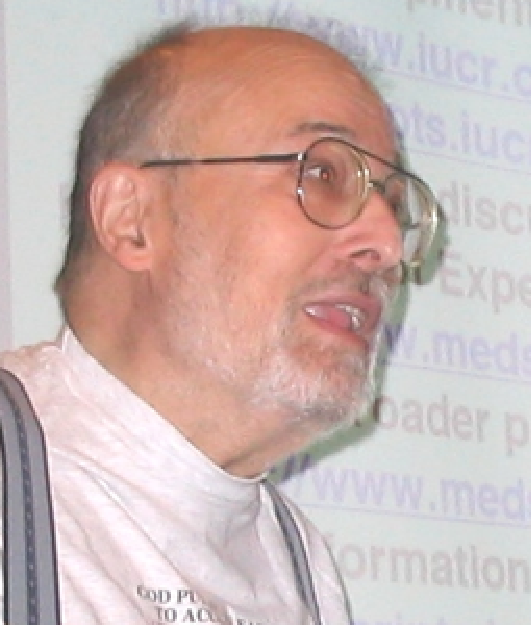
\includegraphics[width=50mm]{Bernstein_Herbert}
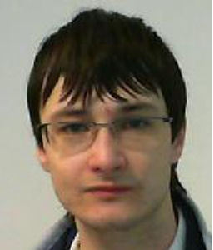
\includegraphics[width=50mm]{Sloan_Jonathan}
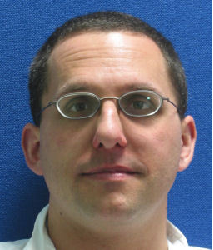
\includegraphics[width=50mm]{Winter_Graeme}
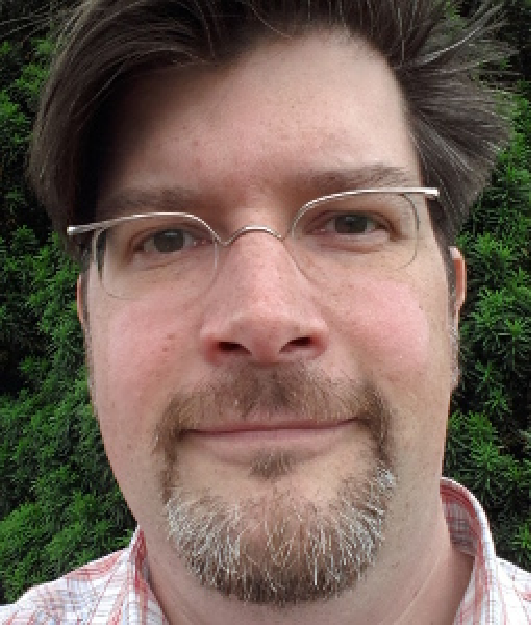
\includegraphics[width=50mm]{Richter_Tobias}
\end{center}
\end{figure}

\end{minipage}\hfill%
\begin{minipage}[]{.4\linewidth}
\begin{center}
\vspace{8mm}

{\fontsize{24}{28}\selectfont $^{\dagger}$Department of Mathematics and Computer Science, Dowling College, Oakdale, NY 11769 (USA)}

{\fontsize{24}{28}\selectfont $^{\star}$Diamond Light Source, Harwell Science and
Innovation Campus, OX11 0DE (UK)}

{\fontsize{24}{28}\selectfont $^{\ddag}${http://wiki.nexusformat.org/NIAC}}

{\fontsize{24}{28}\selectfont $^{\Psi}${http://www.iucr.org/resources/cif/comcifs}}
\vspace{4mm}
\end{center}
\end{minipage}\hfill%
\begin{minipage}[]{.10\linewidth}
\begin{figure}[H]
\begin{center}

\includegraphics[width=50mm]{niac_qr}
{~~\\
NIAC}
\end{center}
\end{figure}
\end{minipage}\hfill%
\begin{minipage}[]{.10\linewidth}
\begin{figure}[H]
\begin{center}

\includegraphics[width=50mm]{comcifs_qr}
{~~\\
COMCIFS}
\end{center}
\end{figure}
\end{minipage}
\\
\fontsize{18}{22}\selectfont
\begin{minipage}[]{0.01\linewidth}~\end{minipage}\hfill\begin{minipage}[]{0.29\linewidth}
\fontsize{18}{22}\selectfont
\begin{figure}[H]
\begin{center}
      {
\fontsize{16}{20}\selectfont ~~\\
Poster T-16 for 11.00 Synchrotron Radiation, Abstract 1388
20 -- 24 July 2013 at American Crystallographic Association meeting, Honolulu, Hawaii.\\
Work supported in part by NIGMS, DOE, NSF, PaNdata ODI (EU 7th Framework Programme)}
\end{center}
\end{figure}

\vspace{-20mm}
\section*{Introduction}

\fontsize{18}{22}\selectfont%
The BIG DATA demands of the new generation of X-ray pixel array
detectors necessitate the use of new storage technologies as we meet
the limitations of existing file systems. In addition, the modular
nature of these detectors provides the possibility of more complex
detector arrays which in turn requires a complex
description of the detector geometry. Taken together these give an
opportunity to combine the best of CBF/imgCIF (the Crystallographic
Binary File), NeXus (a common data format for neutron, x-ray and muon
science) and HDF5 (Hierarchical Data Format, version 5) for the
management of such data at synchrotrons. Discussions are in progress
between COMCIFS (the IUCr Committee for the Maintenance of the CIF
Standard) and NIAC (the NeXus International Advisory Committee) on an
integrated ontology. A proof-of-concept API based on CBFlib and the
HDF5 API is being developed in a collaboration among Dowling College,
Brookhaven National Laboratory and Diamond Light Source. A preliminary
mapping and a combined API are under development.
\begin{itemize}
\item{The new generation of high performance x-ray detectors requires
    integration of HDF5, NeXus and CBF.}
\item{The DECTRIS workshop in Baden, Switzerland in January 2013
    established the parameters of the integration.} 
\item{A collaboration has been working on specifications and code.}
\item{CBFlib 0.9.2.12
\begin{itemize}
\item{Can store arbitrary CBF files in HDF5 and recover them.}
\item{Supports use of all CBFlib compressions in HDF5 files.}
\item{Provides minicbf2nexus to convert sets of minicbf files to a single NeXus file.}
\end{itemize}}
\item{A draft concordance between MX CBF and NeXus has been prepared.}
\item{Updated CBF dictionary has been prepared.}
\item{There is much work still to be done -- collaborators welcome.}
\end{itemize}
\vspace{-8mm}%

\subsection*{Data Rates, Formats and High Performance X-ray Detectors}

\fontsize{18}{22}\selectfont%
CCD X-ray detectors provide images at a moderate data rate of one every
few to several seconds. Current higher performance X-ray detectors, such as the DECTRIS Pilatus
are capable of collecting six-megapixel images at 10 -- 25 frames per
second \cite{Trueb2012}, while the newest Pilatus3 6M instruments can
operate at 100 frames per second. The coming next generation of high performance 
X-ray detectors for MX such as the DECTRIS Eiger will be capable of collecting
16+ megapixel images at more than 125 frames per second \cite[page 6]{Willmott2011} \cite{Johnson2012}.
The ADSC DMPAD \cite{Hamlin2012} is also expected
to produce 900 fine-sliced images in steps of two-tenths of a degree
at 125 frames per second.

%\begin{table}[htdp]
\begin{center}
{\fontsize{20}{24}\selectfont%
 \bf Typical Sustained Data Rates}
\begin{tabular}{lcccc}
\hline
         & {\bf Raw Image}& {\bf Frame}& {\bf Compressed} & {\bf USB Disk}\\
{\bf Detector }& {\bf size (MB) }&{\bf Rate (Hz) }& {\bf Rate (Gb/sec)}& {\bf Data Rate (\%)}\\
\hline
ADSC Q315 (2x2 binned) & 18 MB & 0.37 & .013 & 7 \\
Pilatus 2 6M      & 24& 10 & .48 & 240\\
Pilatus 2 Fast 6M & 24 & 25 & 1.2 & 600\\
Pilatus 6 6M      & 24& 100 & 4.8 & 2400\\
Eiger 16M         &72& 125 & 18& 9000 \\
\hline
\end{tabular}
{\fontsize{16}{20}\selectfont%
\vspace{3mm}\\
Typical sustained data rates for detectors used for MX at NSLS, Diamond Light
Source, etc. compared to expected rates from Eiger, expressed in terms of the 
typical data rate for an inexpensive
USB disk of 25 MB/sec = 200 Mb/sec.} 

\end{center}


Today for MX alone Diamond Light
Source employs one Pilatus 2M, three Pilatus 6M fast and one Pilatus 3
6M, giving a combined data rate of over 1 GB/sec and over 200 files/sec.
These new detectors are creating the need to manage hundreds of thousands of
images being received at rates from sixty megapixels to 2.5 gigapixels per second and beyond.
For the Advanced Beamlines for Biological Investigations with 
X-rays (ABBIX) that are being built for NSLS-II \cite{Hendrickson2012}, just two of the beam lines,
the Frontier Macromolecular Crystallography (FMX) beamline and the Automated Macromolecular Crystallography (AMX) beamline \cite{Schneider2012}, are expected to produce an aggregate of more than 94 terabytes per operational half day,
 660 terabytes per week or 38 petabytes per year.   The anticipated beamline flux is $\mathbf{10^{13}}$ photons per second for FMX and  $\mathbf{2 \times 10^{13}}$ photons 
per second for AMX, approximately 50 times the NSLS X25 and X29 fluxes.  One subtle effect of
these high fluxes is that there will be more photons per pixel in images, making them more
difficult to compress.



\begin{itemize}
\item{A data management system designed for very large numbers of files as well as
for very large data volumes and data rates is needed.}
\item{Efficient recording of metadata coordinated with the data is needed, and database
 access to information about images and experimental runs is needed.}
\end{itemize}
 
\vspace{-6mm}%
\begin{figure}[H]
\begin{center}
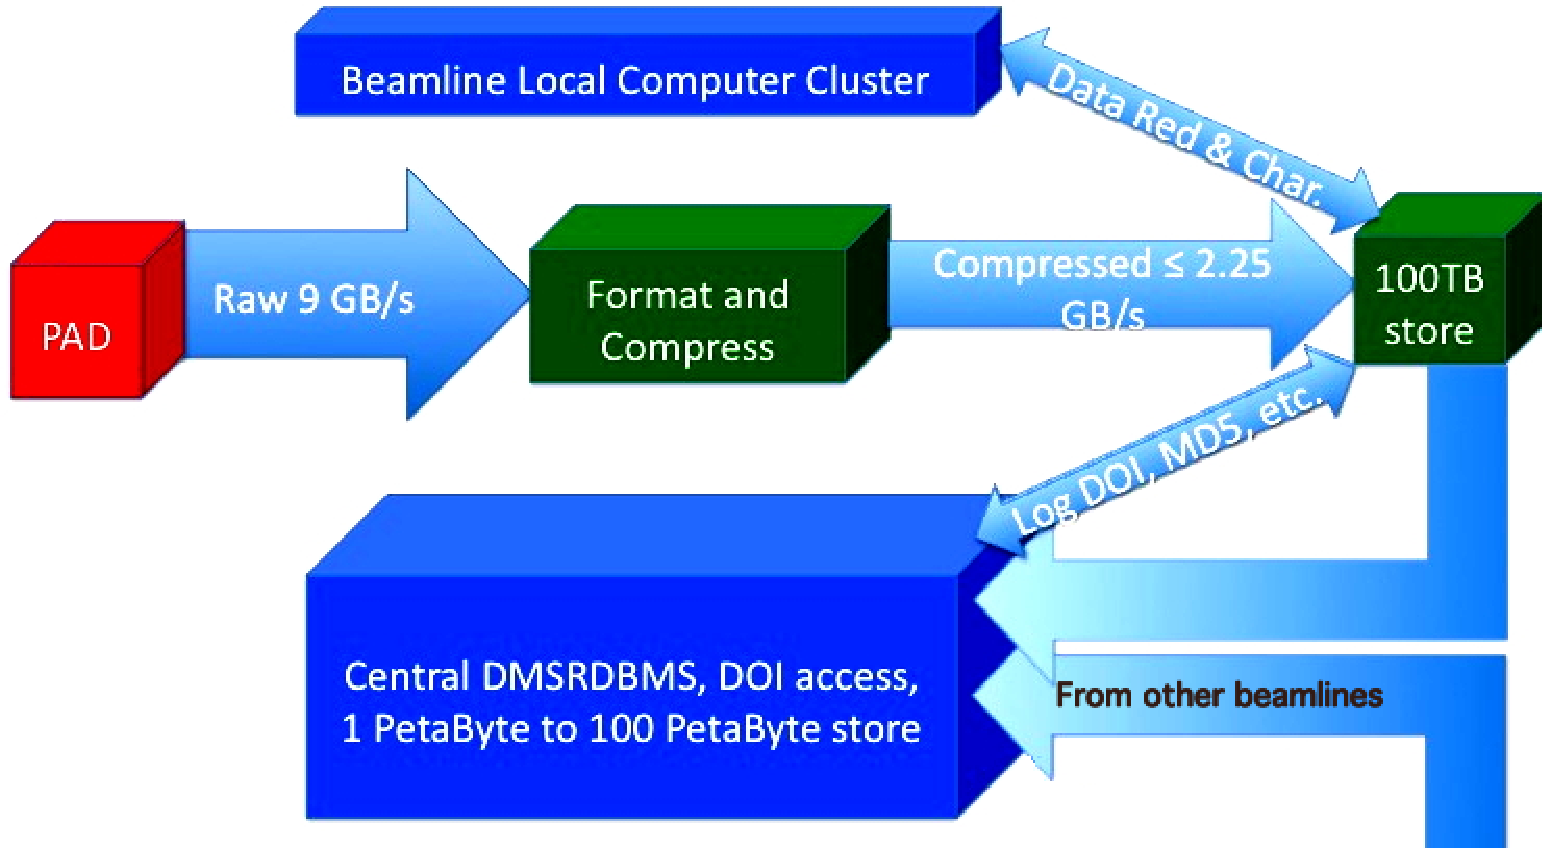
\includegraphics[width=175mm]{PAD_TO_DMSRDBMS_6}
\caption{\fontsize{16}{20}\selectfont%
Major data flows from the beamline advanced pixel array detectors (PADs) to the data
management system relational database (DMSRDBMS).  In order to be manageable, the
raw 9 gigabyte per second data flow from each PAD needs to be compressed locally
by at least 4:1, before going into a beamline 100 terabyte store for beamline local computer cluster
access for up to a week for  data reduction and characterization. 
The required bandwidth of the pipes from the beamlines to the DMSRDBMS depends on the compression used.  
If no further compression is used, 2.25 gigabyte (18 gigabit) per second per beamline network connections are required.  If a combined lossless/lossy compression is used, then 225 -- 450 megabyte (1.8 to 3.6 gigabit) per second per beamline network connections will suffice.  The flows for transfers
to user home institutions are not shown.}
\label{PAD_TO_DMSRDBMS_4}
\end{center}
\end{figure}

\vspace{-4mm}%
\begin{itemize}
\item{For MX, these data rates, data volumes, numbers of distinct images and numbers of distinct experiments argue for a very organized, high performance infrastructure.}
\item{HDF5 and NeXus provide the necessary organization of the raw data.}
\item{CBF provides the necessary organization of the associated metadata for subsequent processing
as well as contributing useful compressions.}
\end{itemize}

A final issue, in addition to the actual recording of data, is that
of automated processing. At Diamond Light Source and elsewhere there
has been a push towards the automated analysis of diffraction data, as
interactively processing diffraction data at the current rate of
typically 20 data sets per hour is unsustainable. This however places an
increased strain on the file system, as typically the same data are read as
many as six times in order to be processed, resulting in over 1000 file access
operations per second. With the storage of many frames per file, as
planned for NeXus, the rate of file operations would decrease substantially.

\vspace{-4mm}%
\subsection*{Where to Find Software and Documentation}

\vspace{-4mm}%
\begin{itemize}
\item{{\bf Draft imgCIF/CBF version 1.7 dictionary} that now includes information on going from CBF to NeXus:

{\fontsize{22}{24}\selectfont \url{https://www.sites.google.com/site/nexuscbf/home/cbf-dictionary}}
}

\item{{\bf PDF summary of the concordance}:

{\fontsize{22}{24}\selectfont \url{https://www.sites.google.com/site/nexuscbf/mapping-draft}}
}

\item{{\bf CBFlib kit:}

{\fontsize{22}{24}\selectfont \url{http://downloads.sf.net/cbflib/CBFlib-0.9.2.12.tar.gz}}

includes both Jonathan Sloan's utility minicbf2nexus to
convert sets of minicbfs into a single NeXus file and
a plugin filter that supports the full set of CBFlib compressions
in HDF5.}
\end{itemize}

\vspace{-5mm}
\begin{minipage}[]{0.29\linewidth}
\begin{center}

\includegraphics[width=50mm]{cbfdic_qr}
{~~\\
CBF dictionary}
\end{center}
\end{minipage}\hfill%
\begin{minipage}[]{0.29\linewidth}
\begin{center}

\includegraphics[width=50mm]{mappingdraft_qr}
{~~\\
CBF-NeXus concordance}
\end{center}
\end{minipage}\hfill%
\begin{minipage}[]{0.29\linewidth}
\begin{center}

\includegraphics[width=50mm]{cbflibdownload_qr}
{~~\\
CBFlib-0.9.2.12 download}
\end{center}
\end{minipage}


\end{minipage}%
\hspace{10mm}\hfill\begin{minipage}[]{0.29\linewidth}



 
% \fontsize{18}{22}\selectfont 
\section*{HDF5 and NeXus}%


\begin{wrapfigure}{r}{0.45\textwidth}
\begin{center}
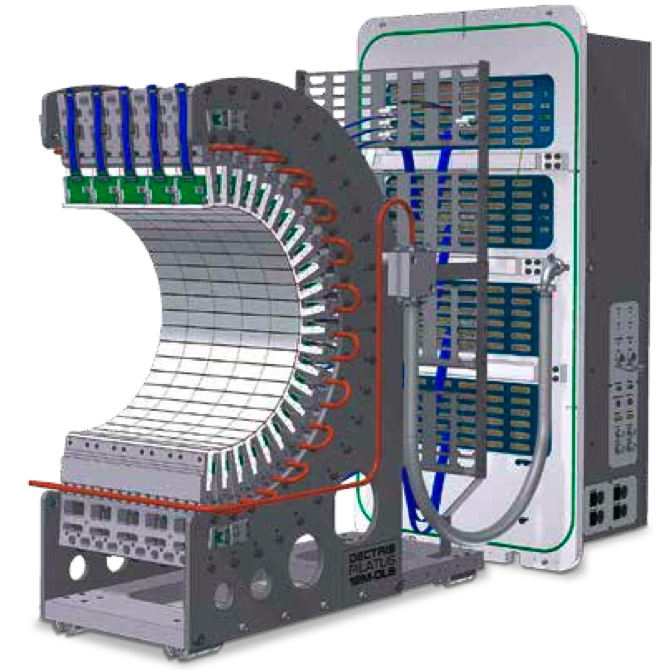
\includegraphics[width=4.5in]{I23}
\caption{\fontsize{16}{20}\selectfont %
Curved DECTRIS detector
for DLS beamline I23, an example of a detector with a complex geometry 
best described using the imgCIF/CBF ontology.
}
\label{fig:i23}
\end{center}
\end{wrapfigure}

The Hierarchical Data Format Version 5 (HDF5) is a self-describing
file format with a robust, well documented API capable of handling
(and routinely used to handle) multi-gigabye files of data.  It has a
diverse user community covering a wide range of disciplines and is 
fully supported \cite{Dougherty2009}. NeXus \cite{Filges2001} is a
tree-oriented view of HDF5 (and XML and HDF4) of importance in
managing neutron and x-ray data.  NeXus is a convenient thin layer
over HDF5 that is widely used at many physics research centers,
including at synchrotrons. Together they provide a portable,
extensible and efficient format for the storage and management of data.
HDF5 is particularly well suited to the management of very large volumes of
complex scientific data and has been adopted as the primary data-management
framework in a wide range of
disciplines\footnote{\url{http://www.hdfgroup.org/HDF5/users5.html}}
and provides the ``inner workings'' of important formats, such as
NetCDF \cite{Rew2004} and NeXus. 

While HDF5 is tree-oriented, which is a very powerful and useful
characteristic allowing file-system-like nesting of groups of data
within groups of data, in order for information to be
easily, reliably and efficiently searched, tables are more useful 
so that the information can be loaded into a relational database
management system \cite{Codd1970}. 


% \begin{figure}[htbp] 
\begin{wrapfigure}{l}{0.45\textwidth}
\begin{center}
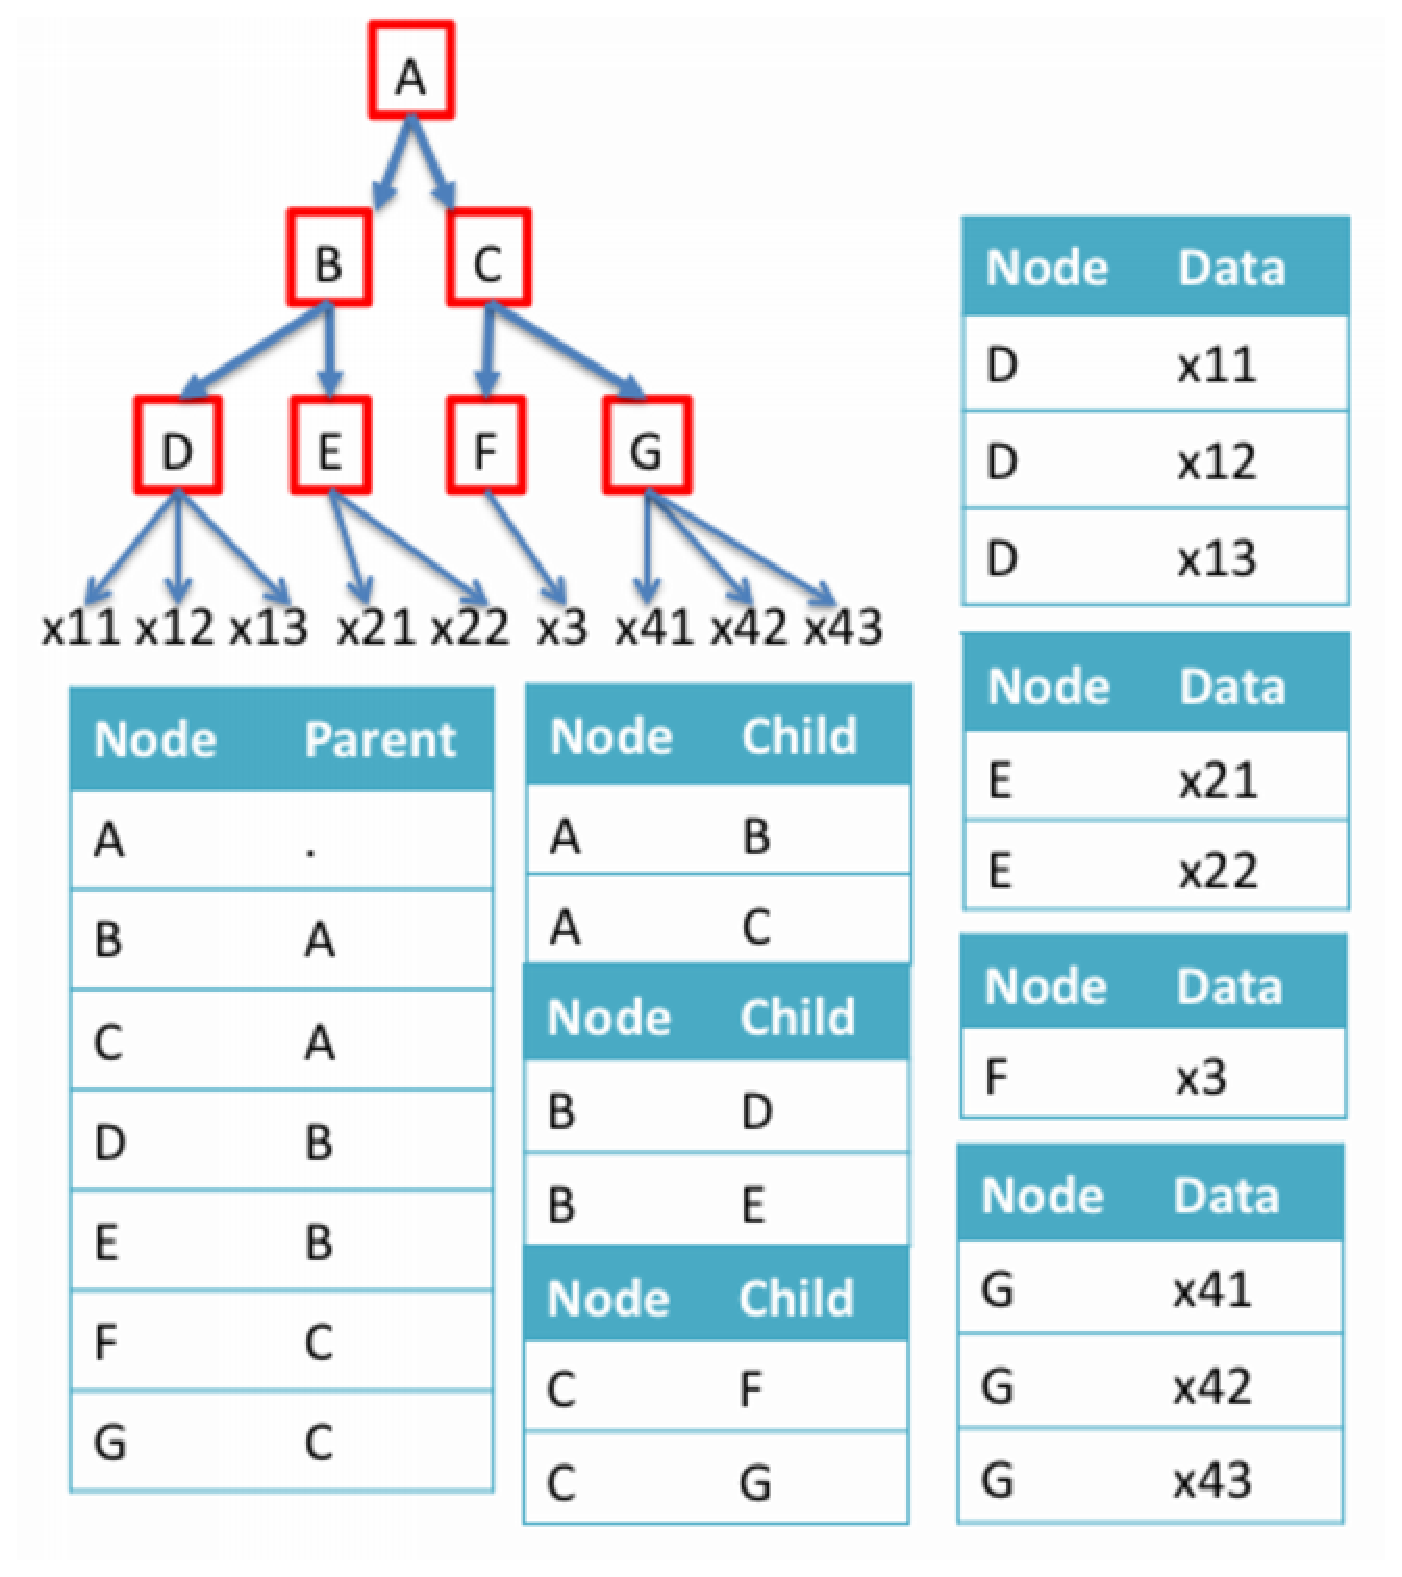
\includegraphics[width=4.25in]{Tree_Example2}
\caption{\fontsize{16}{20}\selectfont %
Example of a tree mapped into tables for database access identifying the links between
parents and children in both directions as well as data.  This is about the simplest example
we can provide of a tree that demonstrates the need for ``normalization'' in the conversion
from trees to tables.}
\label{fig:Tree_Example}
\end{center}
\end{wrapfigure}
%\end{figure}

For this project, organizing data and metadata according to the
conventions of the IUCr Crystallographic Information File
\cite{Hall1991} using imgCIF \cite{imgCIF} and its open source
supporting software CBFlib \cite{CBFlib2005} provides a
database-friendly tabular structure.  The imgCIF ontology provides the
metadata needed for diffraction images and is supported by all the
major detector manufacturers. This aspect is particularly important
for instruments with complex geometries, for example Fig. {\ref{fig:i23}}, a
detector being constructed by DECTRIS for the long wavelength beamline
I23 at Diamond Light Source. 


The embedding of CIF tables in HDF5
files was demonstrated at the  
``HDF5 as hyperspectral data analysis format'' workshop in January 2010. \cite{Gotz2010}  The
workshop recommendation was, in part, ``... Adopt at as much as possible from imgCIF and sasCIF
 \footnote{ \url{http://www-bernstein-plus-sons/software/CBF/doc/cif_img_1.5.4.html}} ...''   There is
 no conflict with the use of HDF5 in this approach.  

\noindent{}Tables are easily embedded into trees.  Going in
the other direction is more difficult.  There
is serious effort required to make general trees into tables suitable for use in a relational
database management system, involving a process known as ``normalization.''  \cite{Codd1972}.
See Fig. \ref{fig:Tree_Example}.
One of the tasks of this project is to extend the imgCIF ontology to ensure workable database
access to metadata in the HDF5 tree that has not already been normalized into CIF categories.
For example, DOIs and SHA2 or SHA3 checksums from multiple experiments will need to be brought
forward into a common table for searching for forensic validation service support.

\section*{CBF and Database Access}%
\fontsize{18}{22}\selectfont %
\noindent{}The Crystallographic Binary File (CBF) format is a complementary format to the Crystallographic 
Information File (CIF), supporting efficient storage of large quantities of experimental data in a 
self-describing binary format \cite{imgCIF}, with a sophisticated
description of the experimental geometry.  For large PAD images, the raw binary CBF format is heavily used both within laboratories and for interchange among collaborating groups.  When dealing with large numbers
of independent experiments producing large numbers of CBF/imgCIF image files, HDF5 provides
the necessary virtual file system needed to manage the massive data flow.  While it is feasible
to simply encapsulate the CBF/imgCIF image files as opaque objects within an HDF5-based
data-management system, active management of the data can be done more efficiently when the
imgCIF tags are made visible in the HDF5 tree, a capability demonstrated in 2010. 
With the anticipated throughput of NSLS II beamlines, and the current
capabilities of MX beamlines equipped with pixel array detectors, the
management of data and the possibility of interrogating the data files
for experimental information becomes critical.


\section*{Compression}
\fontsize{18}{22}\selectfont %
\begin{itemize}
\item{Long-standing issues in Crystallography
\begin{itemize}
\item{High speed, high compression ratio compression is a critical issue for the next generation of detectors.}
\item{Some compressions raise license issues.} 
\item{Some popular compressions are slow or inefficient or both.}
\item{Some compressions can be handed in processing programs such as XDS if license and language issues can be addressed.}
\end{itemize}}
\item{Low pixel density fine-slicing with clean backgrounds makes some compressions more effective.}
\item{CBFlib provides useful compressions.}
\item{A plugin has been written to allow HDF5 to read and write CBFlib compressions.}
\end{itemize}

\begin{figure}[H]
\begin{center}
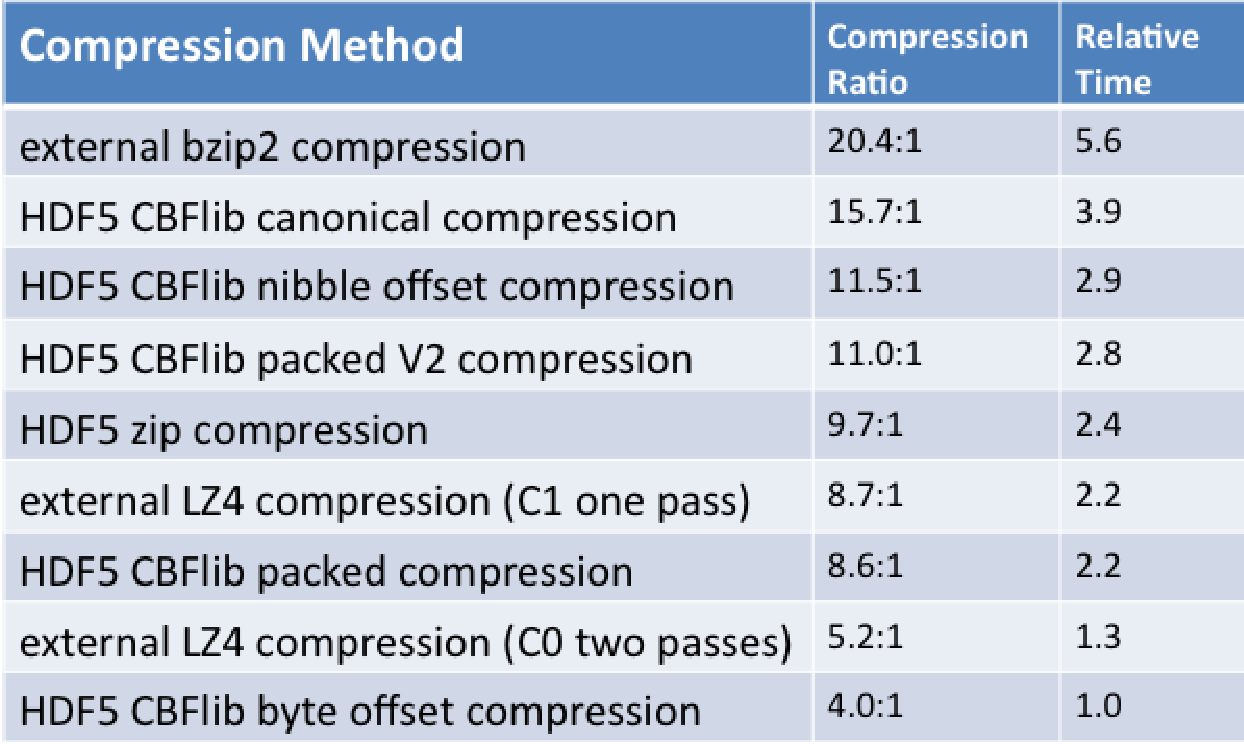
\includegraphics[width=200mm]{Compression_50}
\caption{\fontsize{18}{22}\selectfont%
Tests on fifty X4\_lots\_M1S4\_1\_0???.cbf files from DLS – low to moderate pixel density.   Total size 1.2 gigabytes.  Relative times are shown.  Multiply by 3 for the number of cores needed
to keep up with the compression workload.  The fifty files are from a set of 900 images recorded by Graeme Winter at 
Diamond Light Source beamline I02 as part of routine development work, and come from a crystal of DNA
(TCGGCGCCGA) bound to a large ligand (lambda-[Ru(TAP)2(dppz)]2+).  The aggregate of fifty was chosen
to produce an uncompressed file small enough (1.2 GB) to be acceptable at user sites.  Larger aggregates could
be used for sites able to accommodate large files.}
\label{Compression}
\end{center}
\end{figure}



\subsection*{Jan 2013 DECTRIS Eiger Workshop and Followup}
 
The attendees at the January 2013 DECTRIS Workshop agreed on use of an HDF5-based NeXus format for DECTRIS’ Eiger pixel array detector.

\begin{itemize}
\item{The workshop charged Herbert J. Bernstein with followup on mapping additional terms to the new format.}
\item{Tobias Richter, Jonathan Sloan and Herbert J. Bernstein have worked on a CBF-NeXus concordance and supporting software based on CBFlib and HDF5 with the cooperation of Bob Sweet, Graeme Winter and Mark Koennecke.}
\item{Discussions with NIAC are in progress and discussions with COMCIFS are planned prior to ECM 28 in August 2013.}
\item{Workshop attendees have been sent an updated CBF dictionary and draft CBF-NeXus-HDF5 concordance, as well as a link to a CBFlib-0.9.2.12 kit with minicbf2nexus and a plugin to make CBFlib compression available in HDF5.}
\end{itemize}

 
\end{minipage}\hspace{10mm}\hfill\begin{minipage}[]{0.29\linewidth}

\section*{minicbf2nexus}

\begin{itemize}
\item{Takes some minicbf files and axis configuration settings for them and creates a NeXus file containing the same data. As this is an early version of the program it should not be assumed to be stable.}
\item{-z (or –compression)  \{zlib|none\}\\
\vspace{-2mm}
\noindent{}At present zlib is supported.  CBFlib compressions will follow shortly.}
\vspace{2mm}
\item{-c (or –config) CONFIGFILE\\
\vspace{-2mm}
\noindent{}This takes a single argument giving the file name of a configuration file which describes how the axes of the minicbf file relate to each other.}
\vspace{2mm}
\item{-o (or –output) OUPUTFILE\\
\vspace{-2mm}
\noindent{}Other arguments are interpreted as file names describing the minicbf files to be packed into the new NeXus file.}

\end{itemize}


\section*{CBFlib Compressions from HDF5}

\fontsize{18}{22}\selectfont %
Starting with CBFlib release 0.9.2.11, a plugin module is provided to allow access to CBFlib compressions from HDF5 1.8.11 and later. For general documentation on HDF5 dynamically loaded filters, see 
http://www.hdfgroup.org/HDF5/doc/Advanced/DynamicallyLoadedFilters
/HDF5DynamicallyLoadedFilters.pdf.
The filter has been registered with the HDF5 group as 32006, and cbf.h includes the symbolic name for the filter CBF\_H5Z\_FILTER\_CBF.
The source and header of the CBFlib filter plugin are cbf\_hdf5\_filter.c and cbf\_hdf5\_filter.h, respectively. To use the filter in C applications, you will need to include cbf\_hdf5\_filter.h in the application and have the cbflib.so library in the search path used by HDF5 1.8.11. 

Each compressed image in the HDF5 is in the same format as the MIME-headed compressed images in a CBF, so the Fortran image search logic used in XDS can be used directly on these files.

Typical code:

\begin{verbatim}
unsigned int cd_values[CBF_H5Z_FILTER_CBF_NELMTS];
    hsize_t chunk[3];
    hid_t valspace;
    chunk[0] = 1;  chunk[1] = dimmid; chunk[2] = dimfast;
    cd_values[CBF_H5Z_FILTER_CBF_COMPRESSION] = compression;
    cd_values[CBF_H5Z_FILTER_CBF_RESERVED]    = 0;
    cd_values[CBF_H5Z_FILTER_CBF_BINARY_ID]   = id;
    cd_values[CBF_H5Z_FILTER_CBF_PADDING]     = padding;
    cd_values[CBF_H5Z_FILTER_CBF_ELSIZE]      = (bits+7)/8;
    cd_values[CBF_H5Z_FILTER_CBF_ELSIGN]      = sign;
    cd_values[CBF_H5Z_FILTER_CBF_REAL]        = realarray;
    cd_values[CBF_H5Z_FILTER_CBF_DIMFAST]     = dimfast;
    cd_values[CBF_H5Z_FILTER_CBF_DIMMID]      = dimmid;
    cd_values[CBF_H5Z_FILTER_CBF_DIMSLOW]     = dimslow;
    valprop = H5Pcreate(H5P_DATASET_CREATE);
    H5Pset_chunk(valprop,3,chunk);
    H5Pset_filter(valprop,CBF_H5Z_FILTER_CBF,H5Z_FLAG_OPTIONAL,
        CBF_H5Z_FILTER_CBF_NELMTS,cd_values);
\end{verbatim}

\section*{Nexus -- CBF Concordance}
\begin{itemize}

\item{Mapping from CBF to NeXus
\begin{itemize}
\item{Almost all CBF MX-related categories have proposed slots in the NeXus tree.}
\item{If desired, all CBF data blocks, categories, columns and value will be preserved in
tabular form in the NeXus tree for database use or faithful recovery of the original CBF.}
\end{itemize}}

\item{Mapping from NeXus to CBF
\begin{itemize}
\item{All NeXus base classes have proposed slots in CIF categories.}
\item{Handling of the DECTRIS-proposed Eiger HDF5 format is in the concordance.}
\end{itemize}}

\item{This concordance will require some relaxation of current NeXus name practices.
``CBF\_'' prefixes have been proposed.}

\end{itemize}
\vspace{-6mm}

%\bibliographystyle{plain}
\bibliographystyle{wmaainf}
\bibliography{Integration_Poster}

\vspace{-3mm}
\section*{Acknowledgements}

\begin{itemize}
\item{BNL PXRR Group\\
~~~~Robert M. Sweet, Dieter Schneider, Howard Robinson, John Skinner, Matt Cowan, 
Leonid Flaks, Richard Buono}
\vspace{-2mm}
\item{DLS\\
~~~~Alun Ashton, Bill Pulford}
\vspace{-2mm}
\item{Dowling College ARCiB Lab Group\\
~~~~Mojgan Asadi, Kostandina Bardhi, Maria Karakasheva, Ming Li, Limone Rosa}
\vspace{-2mm}
\item{DECTRIS, BIOIHDF, HDF Group}
\vspace{-2mm}
\item{Frances C. Bernstein}
\vspace{-2mm}
\item{Work funded in part by NIGMS, DOE, NSF, PaNdata ODI (EU 7th Framework Programme)}

\end{itemize}

\end{minipage}\hfill

\vfill
\end{document}  
